\documentclass[11pt]{article}

\usepackage[utf8]{inputenc}
\usepackage[T1]{fontenc}
\usepackage[english]{babel}
\usepackage{geometry}
\geometry{a4paper, margin=2.5cm}
\usepackage{booktabs}
\usepackage{graphicx}
\usepackage{xcolor}
\usepackage{authblk}
\usepackage{amsmath}
\usepackage{float}
\usepackage[numbers,sort&compress]{natbib}
\bibliographystyle{naturemag}
\usepackage[unicode=true,colorlinks=true,linkcolor=blue,citecolor=blue,urlcolor=blue]{hyperref}
\usepackage{lineno}
\linenumbers

\graphicspath{{../figures/}}

\title{\textbf{An Empirically Informed Theory of Paradigmatic Change: Evidence from Public Coverage of Climate Change in Canada}}

\author[1]{Aliz\'{e}e Pillod}
\author[2]{Antoine Lemor}
\author[1]{Matthew Taylor}
\author[1]{Richard Nadeau}
\affil[1]{Universit\'{e} de Montr\'{e}al}
\affil[2]{Universit\'{e} de Sherbrooke}

\date{}

\begin{document}
\maketitle

%TC:ignore
\begin{abstract}
In 1988, Canadian media covered climate change as a scientific problem. By 2023, the worst wildfire season in recorded history produced a political debate about carbon taxes. What changed, and why? Analysing 266,271 articles from 20 Canadian newspapers (1978--2024), we show that climate events are increasingly reinterpreted through political and economic frames. Over four decades, 78\% of causal links between events and media coverage have come to involve a change of frame. The Political-Economic configuration that dominates Canadian climate discourse forms a paradigm that does not need to be actively defended. Meanwhile, Science has lost its dominant position (from 81\% to 23\% of days), its share of media attention (25\% to 11\%), and the voice of its own messengers (39\% to 21\%). The forces most likely to reshape this paradigm are not arguments but events: weather events suppress 71\% of Political cascades, and the accumulation points toward a health-security register.
\end{abstract}
%TC:endignore

%TC:ignore
\vspace{6pt}
\noindent\footnotesize\textit{Word count (main text, excl.\ abstract, captions, references, Online Methods, Supplementary Information):}
\immediate\write18{texcount -1 -sum -merge -q \jobname.tex > \jobname.wcnt}
\input{\jobname.wcnt}
\normalsize
\vspace{12pt}
%TC:endignore

%% ═══════════════ INTRODUCTION ═══════════════

In the summer of 1988, after weeks of heat waves and drought across the Prairies, the \textit{Toronto Star} titled ``Summer of '88 could be hint of the future'' as ``scientists fear warming trend will continue.'' The article featured a researcher explaining that ``the four hottest years in Toronto's history have all been in the 1980s'' and that ``by about 2040 or 2050 we'll be well into it.'' No politician was quoted. The coverage was entirely scientific. Thirty-five years later, in 2023, Canada experienced its worst wildfire season in recorded history. The fires were extensively covered, but the media discussion rapidly shifted toward politics. The \textit{Globe and Mail} reported that ``Poilievre seizes the moment on Atlantic Canada carbon-tax fears'' while the \textit{National Post} declared ``Carbon tax is a loser for Liberals.'' In both cases, the same physical reality, heat waves, droughts and fires, were interpreted through radically \emph{different frames}. 

Entman\cite{entmanFramingClarificationFractured1993} defines framing as the selection and salience-enhancement of particular aspects of perceived reality that promote specific problem definitions, causal interpretations, and policy prescriptions, be they political, scientific, economic, or otherwise. Frames reflect who holds discursive authority, what causal stories circulate, and which policy responses appear legitimate. In 1988, scientists were the main actors to frame and define the problem because they were the only actors who understood it. By 2023, the same physical reality had become a political and economic problem, and the actors who dominated it had changed accordingly. Frames that are dominant thus reveal the paradigmatic structure not only of media discourse, but of the broader forces of society. Frame dominance is therefore a form of discursive power\cite{mccombsAgendaSettingFunctionMass1972, nisbetCommunicatingClimateChange2009}. 

In the public sphere, frames coexist. A single article on climate change may use several frames, and invoke politics, economics, and science simultaneously. But discursive space is finite, and a few frames tend to dominate at the expense of others. The same article may speak of costs and political strategy, but rarely of the rights of displaced populations or of cultural practices in the face of environmental change \emph{at the same time}. When two or three frames are repeated consistently across articles, outlets, and decades, they form a near-permanent structure: a \emph{paradigm}. It is this paradigm that confers discursive power. Hall\cite{hallPolicyParadigmsSocial1993} defines a paradigm as the overarching framework of ideas and standards that structures how a problem is conceived, which solutions are considered, and which actors are legitimate to define the terms of the debate.

Empirical evidence from Canada points toward a political-economic paradigm in climate discourse. Canadian coverage tends to respond to political events rather than ecological conditions\cite{stoddartCanadianNewsMedia2016, schaferWhatDrivesMedia2014, haseClimateChangeNews2021} and to be framed as a governance issue\cite{ahchongAnthropogenicClimateChange2012}. Yet no theory has operationalised a paradigm in a way that makes it measurable, and no empirical framework has proposed mechanisms informed by data rather than postulated. Understanding such a paradigm is essential because it determines who speaks with authority on climate change, which solutions remain conceivable, and whether scientific knowledge can still influence public action\cite{skogstadPolicyParadigmsTransnationalism2011}. \emph{What is the structure of the climate paradigm, how has it changed over half a century, and what mechanisms sustain it?}

%TC:ignore
\begin{figure}[b!]
\centering
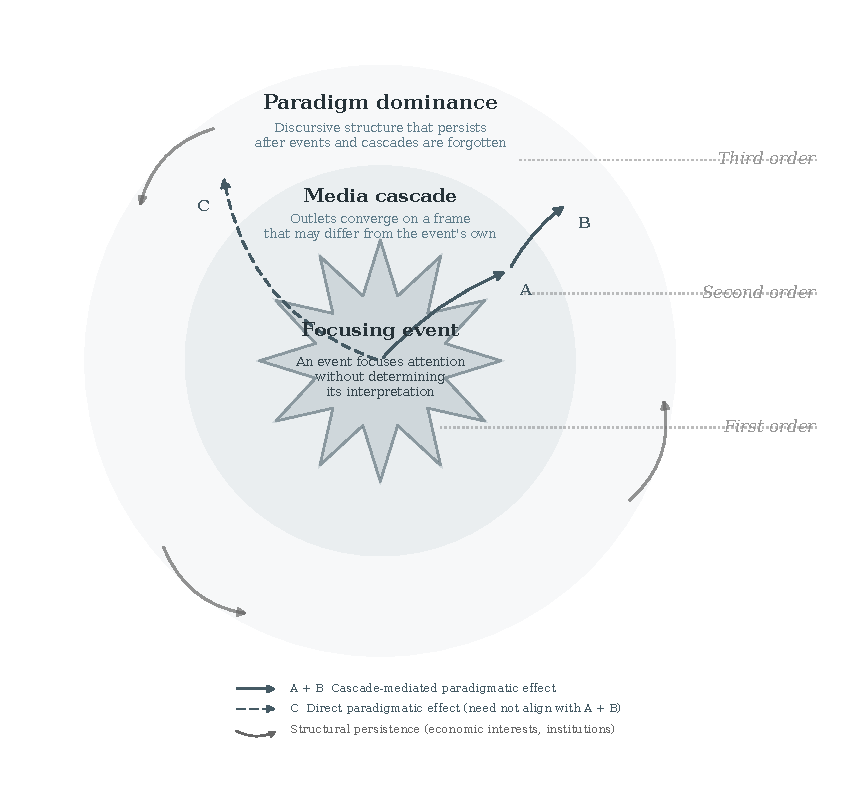
\includegraphics[width=0.72\textwidth]{figure1_schema.pdf}
\caption{\textbf{Three orders of discursive change}, extending Hall\cite{hallPolicyParadigmsSocial1993} from policy to public discourse. A focusing event occurs and focuses attention without determining its interpretation (first order). The media cascade converges on a frame that may differ from the event's own (second order), reinforcing or eroding the existing paradigmatic configuration (third order). A and B represent cascade-mediated paradigmatic effects; C represents the direct paradigmatic effect of events. The two need not align. The paradigm also persists through structural inertia (economic interests, institutional routines) that operates independently of individual events and cascades.}
\label{fig:schema}
\end{figure}
%TC:endignore

We propose a theory organised around three analytically distinct orders of discursive change, extending Hall's\cite{hallPolicyParadigmsSocial1993} three orders of policy change to public discourse. In the spirit of Ockham's razor, the theory can be stated simply (see Fig.~\ref{fig:schema}). A paradigm is the configuration of dominant frames at a given moment. When an event occurs (first order), it can be interpreted through fundamentally different frames. The media converge on one or several dominant interpretations such as a political-economic one, forming a cascade (second order) that either reinforces or erodes the existing paradigm (third order). The paradigm also persists through its own \emph{structural inertia}, independently of any event, sustained by forces such as economic interests or institutions\cite{baumgartnerAgendasInstability2009}.

Each order draws on a distinct body of literature. The first order is the \textit{focusing event}, defined by Birkland\cite{birklandDisasterAgendaSetting1997} and Kingdon\cite{kingdonAgendasAlternativesPublic2014} as an event that reaches the public and elites and opens a window of opportunity for reframing\cite{downsEcologyIssueAttention1972}. Each focusing event enters public attention with a ``natural'' frame. For example, a wildfire is environmental, a COP meeting is political. Yet the event does not determine its media framing. As our first example showed, heat waves and fires can be framed as a political or a scientific problem. 

The second order is the \textit{media cascade}, a period in which multiple outlets converge on the same interpretive frame, creating a self-reinforcing dynamic analogous to the informational cascades described by Bikhchandani et al.\cite{bikhchandaniTheoryFadsFashion1992}. The cascade frame may differ from the event's natural frame because of frame competition\cite{snidermanStructurePoliticalArgument2004} and the politicisation of climate discourse\cite{chinnPoliticizationPolarizationClimate2020, bolsenUSNewsMedia2018}. The event triggers a cascade, but does not control it, and can affect directly the paradigm with or without media cascading effects (Fig.~\ref{fig:schema}). 

The third order is the \textit{paradigm} itself. A cascade can reinforce or erode the existing paradigmatic configuration, but the paradigm is not the direct product of any single event or cascade. It persists long after events and cascades are forgotten, sustained by structural forces such as economic interests that benefit from a particular framing without actively promoting it\cite{culpepperQuietPoliticsBusiness2011}, or the absorption of environmental discourse into economic rationality\cite{hajerPoliticsEnvironmentalDiscourse1995}.

We operationalise this theory using the CCF database\cite{lemorCCFDatabase2026}: 266,271 articles from 20 Canadian newspapers (1978--2024), processed into 9.2 million bilingual sentences with 65 hierarchical annotations (F1=0.866), including eight interpretive frames (Political, Economic, Scientific, Environmental, Justice, Cultural, Health, Security), messengers, event types, and solutions. Sentence-level annotation allows us to measure the recurrence of a particular frame across outlets and over time, and therefore the structure of a paradigm. Canada is simultaneously a major fossil fuel producer and a signatory of every major climate agreement, so that political and scientific framings are structurally in tension. Focusing events are detected through agglomerative clustering on sentence-level embeddings (50,880 event clusters; see \hyperref[sec:methods]{Methods}). Media cascades are detected via PELT changepoint detection on five daily Z-scores. Paradigm dominance is measured using four complementary methods (information theory, network centrality, Granger causality, proportional prominence); a frame achieves dominant status when selected by at least three of four threshold criteria. Causal relationships are identified using stability selection\cite{meinshausenStabilitySelection2010} with Newey-West HAC inference, yielding 9,548 significant effects across the three orders (see \hyperref[sec:methods]{Methods} for full details). The codebase is publicly available.

%% ═══════════════ RESULTS ═══════════════

\section*{Results}

\subsection*{A locked paradigm: politics and economics in, science and environment out}

%TC:ignore
\begin{figure}[b!]
\centering
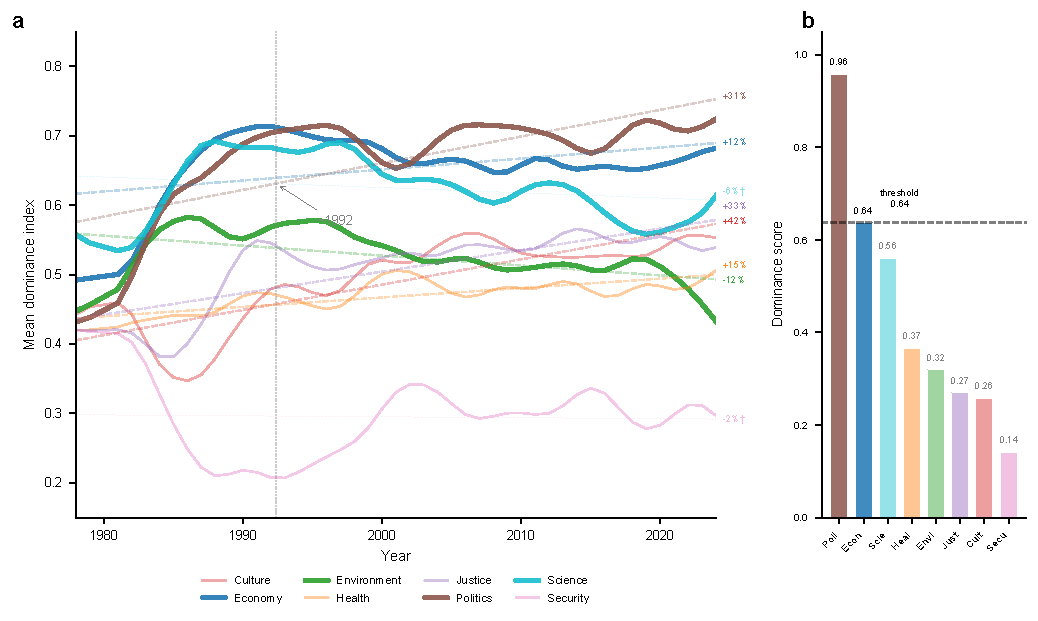
\includegraphics[width=0.95\textwidth]{figure2_paradigm.pdf}
\caption{\textbf{The paradigmatic structure.} (a) Mean paradigm dominance indices by year (smoothed), with linear trend lines for frames with significant slopes ($p < 0.05$). Politics ($+44\%$) and Economy ($+22\%$) rise; Science ($-33\%$) and Environment ($-32\%$) decline. The crossing point at $\sim$1988 marks the transition from scientific to political dominance. (b) Composite dominance score (4-method consensus: information theory, network centrality, Granger causality, proportional prominence). The threshold (0.584) separates the two dominant frames (Politics, Economy) from Science (0.560), which falls just below.}
\label{fig:paradigm}
\end{figure}
%TC:endignore

Two dominant frames were identified across 47 years: \emph{Politics} (composite score 0.925) and \emph{Economy} (0.584). \emph{Science} (0.560) falls just below the dominance threshold (Fig.~\ref{fig:paradigm}b). This structure has not always prevailed. In the early 1980s, \emph{Science} held the highest dominance index, reaching 0.66 in 1982 (Fig.~\ref{fig:paradigm}a). The turning point came in 1988, when \emph{Politics} overtook \emph{Science}. In an article extracted from the database dated June 24, 1988, Howard Ferguson, assistant deputy minister at Environment Canada, declared at the World Conference on the Changing Atmosphere that climate change was ``not just a scientific problem anymore'' and that Canada ``must look at how it will affect lifestyles and standard of living.''

The secular trends confirm this shift (Fig.~\ref{fig:paradigm}a). Over 46 years, \emph{Politics} rose from 0.56 to 0.81 ($+44\%$, $R^2 = 0.42$), while \emph{Science} declined from 0.66 to 0.44 ($-33\%$, $R^2 = 0.56$) and \emph{Environment} from 0.50 to 0.34 ($-32\%$, $R^2 = 0.50$). At the 1992 Rio Summit, Maurice Strong warned that ``the Earth has cancer'' (\textit{Globe and Mail}, May 2, 1992), yet the summit's lasting effect was to recast the environmental crisis as an economic negotiation. \emph{Economy} rose steadily ($+22\%$, $R^2 = 0.22$). In the 1980s, \emph{Science} was dominant on 81\% of days and \emph{Politics} on only 72\%; by the 2020s, \emph{Politics} or \emph{Economy} are dominant every single day, while \emph{Science} retains dominance on only 23\%\cite{youngRepresentationsClimateChange2011} (\hyperref[tab:si_dominance_decades]{Supplementary Table~1}).

\subsection*{First order: the growing distance between events and their coverage}

Four results characterise the first order. The primary is an increasing \emph{frame displacement}. When a focusing event triggers a media cascade, the cascade's frame need not match the event's ``natural'' frame. When in 2016 a wildfire destroyed a town at Fort McMurray, the \textit{Toronto Star} asked ``will Fort McMurray wildfires tip the pipeline debate?'' (May 11, 2016). An environmental event was thus reframed as a political one. Across the full period, 78\% of event-to-cascade links involve such displacement (\hyperref[tab:si_displacement]{Supplementary Table~2}), and this proportion has increased over time, from 71\% to 84\% ($R^2 = 0.17$; Fig.~\ref{fig:displacement}a). 

The second result is a  \emph{declining driver ratio}. Not all causal links between events and cascades are amplifying, as some events may actually suppress and mute an ongoing cascade. In November 2007, the release of the IEA World Energy Outlook and the IPCC synthesis report suppressed an ongoing political cascade on party environmental platforms. The \textit{Calgary Herald} warned of ``no quick fix for global meltdown'' (November 10, 2007) and displaced the partisan debate. Over the full period, the share of amplifying links (driver ratio) fell from 90\% to 46\% ($R^2 = 0.61$; Fig.~\ref{fig:displacement}a, \hyperref[tab:si_displacement]{Supplementary Table~2}). 

Displacement and the driver ratio cross at the end of the 1990s (Fig.~\ref{fig:displacement}a). Before that point, events were more aligned with their natural frame. In 1988, the \textit{Globe and Mail} covered droughts and floods as ``chaotic summer adds fuel to doomsayers' fears'' (September 17, 1988), entirely in an environmental register. After the crossing, events suppress existing cascades as often as they amplify them. This transition coincides with the consolidation of the Political-Economic paradigm (Fig.~\ref{fig:paradigm}a). Once locked in, events are processed through dominant frames rather than through the frame closest to the event itself.
%TC:ignore
\begin{figure}[b!]
\centering
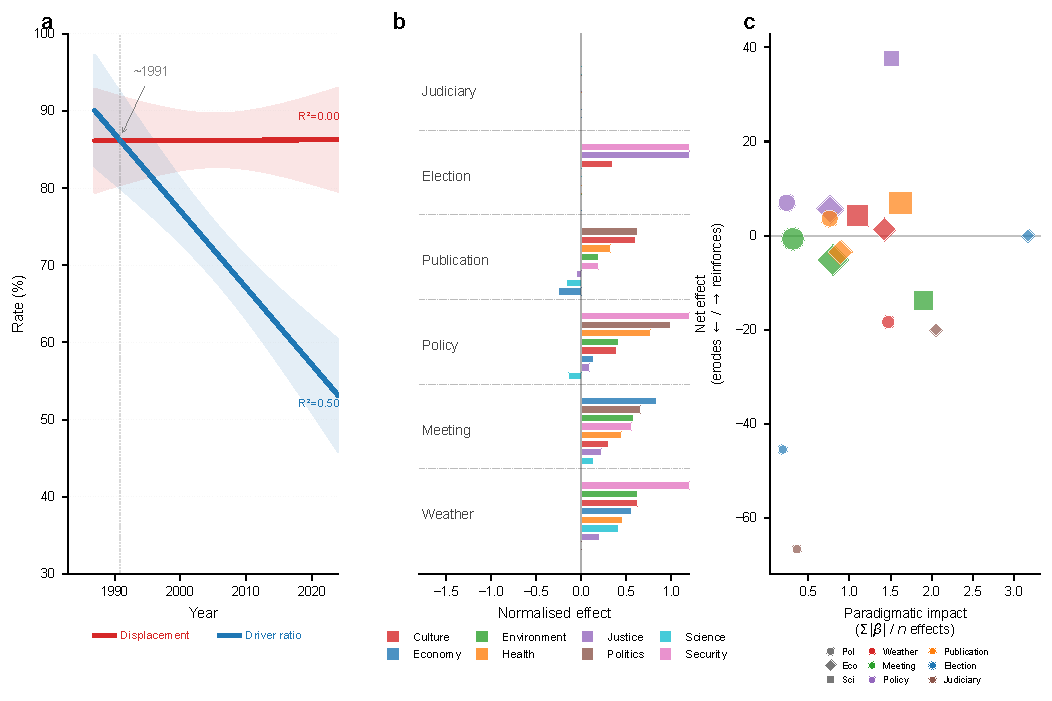
\includegraphics[width=0.95\textwidth]{figure3_first_order.pdf}
\caption{\textbf{First order: frame displacement.} (a) Frame displacement rate (red, 71\% to 84\%, $R^2 = 0.17$) and driver ratio (blue, 90\% to 46\%, $R^2 = 0.61$) with 95\% confidence bands. The two trends cross around 1999. (b) Normalised causal effect of the six main event types on the eight cascade frames (median $\beta$ divided by frame-specific median $|\beta|$). Bars sorted by effect size. Cultural ($n = 66$) and protest ($n = 9$) events are excluded due to insufficient sample sizes, which prevent reliable per-frame estimation; their aggregate effects are reported in \hyperref[tab:si_event_frame]{Supplementary Table~3}. (c) Paradigmatic impact ($\Sigma|\beta|/n$, $x$-axis) versus net paradigm effect (\% catalyst $-$ \% disruptor, $y$-axis) for each combination of event type (colour) and target frame (shape: circle = Politics, diamond = Economics, square = Science). Weather strongly reinforces Politics (red circle, $+33$). Elections strongly erode Economics (blue diamond, $-45$). Most event types cluster near zero net effect, indicating paradigm resistance.}
\label{fig:displacement}
\end{figure}
%TC:endignore

The third result is \emph{attentional redirection} (Fig.~\ref{fig:displacement}b, \hyperref[tab:si_event_frame]{Supplementary Table~3}). Weather events suppress 71\% of \emph{Political} cascades and 52\% of \emph{Economic} ones, but only 17\% of \emph{Security} and 24\% of \emph{Environment} cascades. When the 2021 heat dome killed hundreds in British Columbia, the \textit{Globe and Mail} led with ``B.C.\ records hundreds of deaths linked to heat wave'' (July 1, 2021), entirely in a health register with no political framing. Counter-intuitively, elections also suppress 62\% of \emph{Political} cascades: the frame is so dominant that elections open space for other perspectives, such as \emph{Justice} and \emph{Environment}. Meetings amplify all frames at similar rates (55--75\%), while judiciary events amplify \emph{Science} (75\%) and \emph{Environment} (67\%).

The fourth result is a \emph{decoupling} between cascade-level and paradigmatic effects (Fig.~\ref{fig:displacement}c, \hyperref[tab:si_paradigm_impact]{Supplementary Tables~4--5}). Weather events suppress 71\% of \emph{Political} cascades, yet 67\% of their paradigmatic effects on \emph{Politics} are catalytic ($\bar{\beta}_{0\text{--}2} = +2.31$; \hyperref[tab:si_lag_analysis]{Supplementary Table~5}). After the 2013 Alberta floods, the \textit{Globe and Mail} noted that ``Canada's disaster policy framework is a cat's cradle of perverse incentives'' (June 27, 2013): the flood displaced the carbon pricing debate but raised a structurally larger political question. Elections erode \emph{Economic} paradigm dominance (73\% disruptor): during the 2008 campaign, sentences on ``carbon tax'' were 95\% politically framed but only 10\% economically framed, down from 39\% outside the election period (\hyperref[tab:si_sentence_framing]{Supplementary Table~6}).

%TC:ignore
\begin{figure}[b!]
\centering
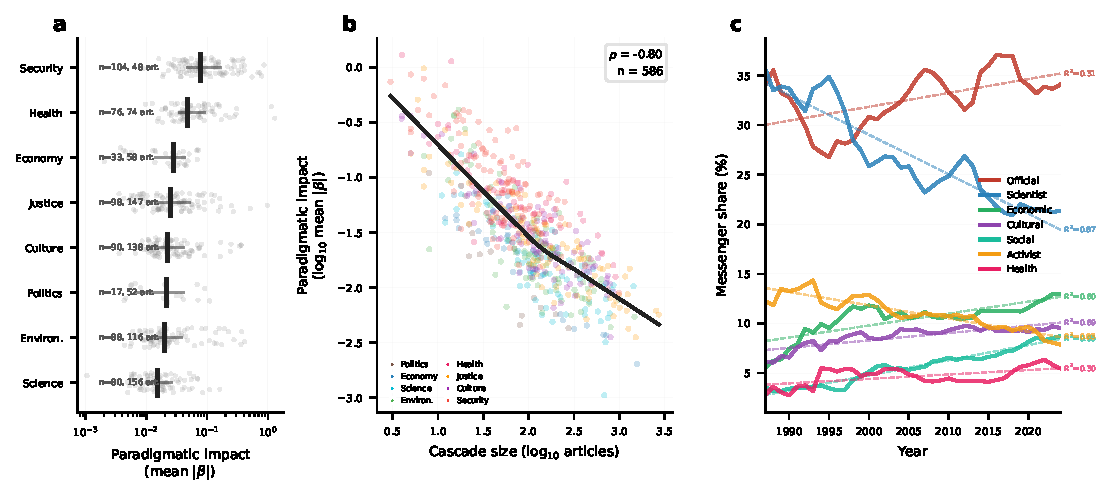
\includegraphics[width=0.95\textwidth]{figure4_second_order.pdf}
\caption{\textbf{Second order: cascades and the paradigm.} (a) Paradigmatic impact (mean $|\beta|$, log scale) by cascade frame. Each point is one cascade ($n = 975$). Median bar and IQR in black. Frames ordered by decreasing impact. Non-dominant frames produce significantly higher impact (partial $\rho = -0.60$ after controlling for size). (b) Cascade size versus paradigmatic impact ($\rho = -0.85$, $p < 10^{-272}$) with LOWESS smooth, coloured by frame. The largest cascades are paradigmatically inert. (c) Messenger share in cascades over time (5-year rolling mean). Scientific messengers declined from 37\% to 18\% ($-0.49$ pp/yr, $R^2 = 0.80$) while official and economic messengers rose.}
\label{fig:secondorder}
\end{figure}
%TC:endignore

\subsection*{Second order: the paradox of media attention without paradigmatic influence}

Four results characterise the second order. The first is \emph{structural inertia}. Of 975 cascades with significant paradigmatic effects, those belonging to \emph{Political} and \emph{Economic} frames produce five times less impact than non-dominant frames (median $|\beta| = 0.009$ vs $0.044$, $p < 10^{-41}$; Fig.~\ref{fig:secondorder}a, \hyperref[tab:si_dominance_impact]{Supplementary Table~10}). This holds after controlling for cascade size (partial $\rho = -0.60$, $p < 10^{-96}$). The dominant paradigm does not need strong cascades to sustain itself. \emph{Economy} is dominant on 85\% of days yet has produced zero strong cascades across 47 years (\hyperref[tab:si_cascade_class]{Supplementary Table~7}). Each sentence is also annotated with the type of actor who speaks (official, scientist, economic actor, activist, among others). Even within \emph{Economic} cascades, economic messengers account for only 19\% of voice share, behind officials (37\%; \hyperref[tab:si_messenger_share]{Supplementary Table~11}). Four of the six largest cascades, all \emph{Political}, produced zero significant paradigmatic effects (Fig.~\ref{fig:secondorder}b, \hyperref[tab:si_largest_cascades]{Supplementary Table~8}). The largest mobilised 6,525 articles across 18 outlets over 94 days in early 2007, yet the configuration of dominant frames remained unchanged.

The second result is a \emph{messenger displacement}. Over 47 years, the share of scientific messengers in cascades fell from 37\% to 18\% ($-0.49$ pp/yr, $R^2 = 0.80$), while official messengers rose from 28\% to 36\% ($+0.20$ pp/yr, $R^2 = 0.72$) and economic messengers from 7\% to 15\% ($+0.18$ pp/yr, $R^2 = 0.65$; Fig.~\ref{fig:secondorder}c, \hyperref[tab:si_messenger_share]{Supplementary Table~11}). The displacement is sharpest within \emph{Science} cascades themselves. In 1984--1995, scientists accounted for 47\% of messenger share in Science cascades and officials for 25\%. By 2016--2024, officials had overtaken scientists (30\% vs 30\%; \hyperref[tab:si_messenger_share]{Supplementary Table~11}). When the \textit{Whitehorse Daily Star} declared ``climate science indisputable'' (November 9, 2015), the speaker was Environment Minister Catherine McKenna, not a scientist. Science is increasingly narrated by officials\cite{hallSocialProductionNews1978} rather than by the scientists who produce it.

The third result is a \emph{cascade capture}. \emph{Political} cascades absorb a growing share of all cascade articles, rising from 22\% in the 1980s to 35\% in the 2020s ($+0.50$ pp/yr, $R^2 = 0.44$), while \emph{Science} cascades fell from 25\% to 11\% ($-0.78$ pp/yr, $R^2 = 0.39$; \hyperref[tab:si_cascade_share]{Supplementary Table~9}). This trajectory mirrors the paradigmatic dominance trends (Fig.~\ref{fig:paradigm}a). The two declines of \emph{Science}, one in paradigm dominance and one in cascade share, reinforce each other. \emph{Science} is losing both its structural force within the paradigm and its capacity to produce the cascade events that could restore it.

The fourth result is a \emph{peripheral accumulation}. The cascades with the highest paradigmatic impact belong to \emph{Security} (median $|\beta| = 0.112$), \emph{Health}\cite{pillodReframingClimateChange2021} ($0.065$), and \emph{Justice} ($0.051$), all non-dominant frames (Fig.~\ref{fig:secondorder}a). These cascades are small (median 24 to 78 articles) but they operate on registers where perceived urgency is high. In 2007, the \textit{Edmonton Journal} reported that ``retired U.S. admirals and generals'' warned of a ``continental security threat'' from an ``ice-free northern sea'' (May 11, 2007). As shown at the first order, weather events suppress \emph{Political} cascades but amplify \emph{Security} (83\% driver rate) and \emph{Health} (71\%). Each of these small peripheral cascades individually produces a larger paradigmatic effect than the largest political mega-cascade. Whether their cumulative pressure can eventually destabilise the dominant configuration remains an open question, but the direction of accumulation is clear.

\subsection*{Third order: displaced chains and the erosion of science}

Three results characterise the third order. The first is that \emph{reframing amplifies paradigmatic effects}. Of 3,012 complete triple chains (event $\to$ cascade $\to$ paradigm), 78\% involve frame displacement between the event and the cascade it triggers (\hyperref[tab:si_triple_stats]{Supplementary Table~12}). Displaced chains produce 80\% more paradigmatic impact than aligned ones (median $|\beta| = 0.029$ vs $0.016$, $p < 10^{-28}$; Fig.~\ref{fig:thirdorder}a). The most consequential pathways involve securitisation\cite{buzanSecurityNewFramework1998, detrazRethinkingEnvironmentalSecurity2009}: weather events reframed through \emph{Security} cascades produce paradigmatic effects seven times larger than the global mean (Fig.~\ref{fig:thirdorder}b, \hyperref[tab:si_triple_stats]{Supplementary Table~12}).

The second is that \emph{the net direction of triple chains sustains the dominant paradigm}. \emph{Politics} is the frame closest to net reinforcement across all cascade channels (47\% catalyst, CI [43, 52]; Fig.~\ref{fig:thirdorder}c, \hyperref[tab:si_triple_stats]{Supplementary Table~12}). The most common pathway routes political events through \emph{Economic} cascades toward \emph{Science} erosion (Meeting $>$ Eco $>$ Sci, $n = 40$, 40\% catalyst). \emph{Economy} and \emph{Culture} are significantly eroded (43\% catalyst). The triple-chain system thus funnels discursive energy toward the Political frame while dispersing it away from its co-dominant partner.

%TC:ignore
\begin{figure}[t!]
\centering
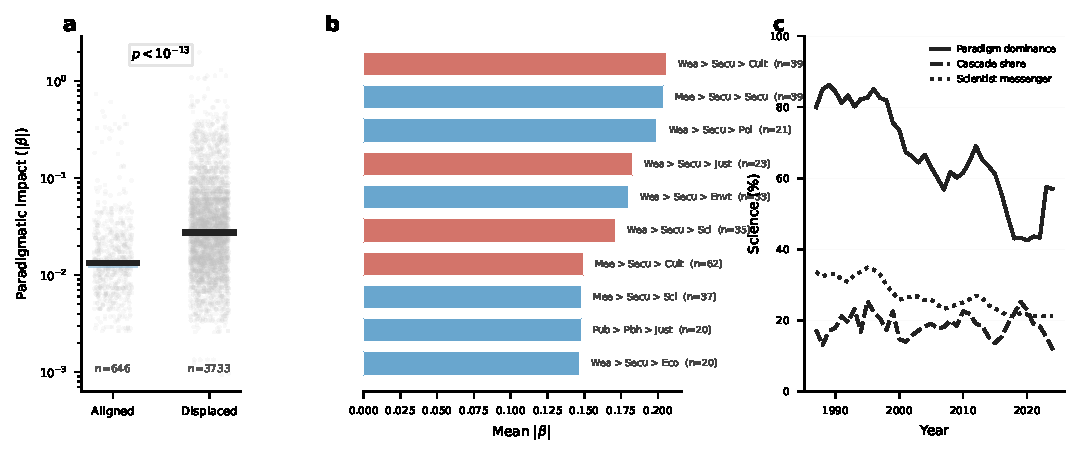
\includegraphics[width=0.95\textwidth]{figure5_third_order.pdf}
\caption{\textbf{Third order: the paradigm as structural residue.} (a) Displaced triple chains (where the cascade frame differs from the event's natural frame) produce 80\% more paradigmatic impact than aligned chains ($p < 10^{-28}$). Coloured rectangles show the bootstrap 95\% CI on the median. (b) Top pathways by paradigmatic impact (mean $|\beta|$). Weather events reframed through \emph{Security} cascades dominate. Red bars indicate net disruption ($<$ 50\% catalyst), blue bars net reinforcement. (c) Scientific dispossession across three measures (5-year rolling mean): paradigm dominance (\% of days), cascade share (\% of articles), and scientist messenger share all decline.}
\label{fig:thirdorder}
\end{figure}
%TC:endignore

The third result is a \emph{scientific dispossession} that converges across all three orders (Fig.~\ref{fig:thirdorder}c). At the paradigmatic level, \emph{Science} dominance fell from 80\% to 23\% of days (Fig.~\ref{fig:paradigm}a). At the cascade level, its share dropped from 25\% to 11\% while officials overtook scientists as narrators of science itself (Fig.~\ref{fig:secondorder}c). At the triple-chain level, the most common pathway erodes \emph{Science} (Meeting $>$ Eco $>$ Sci, 60\% disruptor). The 2023 wildfire season illustrates this convergence. 18 million hectares burned, the largest cascade comprised 3,256 political articles, and the \textit{National Post} opened with ``here comes Ottawa's second carbon tax'' (June 1, 2023). The two \emph{Science} cascades (1,318 articles) produced zero effects on \emph{Science} dominance.

%% ═══════════════ DISCUSSION ═══════════════

\section*{Discussion}

\subsection*{Scientific dispossession as structural displacement}

The political-economic paradigm documented here reflects structural forces in society rather than just editorial choices. Scientists were the first to attract public attention to climate change, but once political actors seized the issue, discursive space was progressively absorbed by political and economic framing. Officials now narrate science on their behalf\cite{hallSocialProductionNews1978}, cascades in the scientific frame have shrunk to 11\% of all coverage, and even the largest mobilisation of scientific articles produces no measurable effect on paradigmatic structure. The "quiet politics" of economic framing\cite{culpepperQuietPoliticsBusiness2011} reinforces this displacement. \emph{Economy} is dominant on 85\% of days without ever producing a strong cascade, ensuring that ``how much does it cost?'' accompanies every climate debate.

\subsection*{Anomalies and the prospect of paradigmatic change}

In Kuhn's\cite{kuhnStructureScientificRevolutions1996} account, paradigms fall to the accumulation of anomalies that the dominant framework cannot absorb. Our data suggest an analogous process. Weather events, the physical anomalies of climate change, suppress 71\% of \emph{Political} cascades and, when reframed through \emph{Security}, produce paradigmatic effects seven times larger than the global mean. The direction of this accumulation points toward a health-security register. \emph{Security} and \emph{Health} cascades already produce the highest paradigmatic impact of any frame, consistent with the argument that climate change is fundamentally a health crisis\cite{costelloManagingHealthEffects2009, romanelloLancetCountdown2023}. If extreme weather events continue to intensify, the discursive pressure may eventually reshape the paradigm toward a configuration in which bodily harm and territorial security, not carbon pricing, define the terms of the debate.

Elections constitute a different source of disruption. They suppress 62\% of \emph{Political} and 72\% of \emph{Economic} cascades, and erode \emph{Economic} paradigm dominance (73\% disruptor). Unlike weather events, which accumulate in a single direction, elections open discursive space across multiple frames at once and could constitute moments of paradigmatic rupture.

\subsection*{Limitations}

Our analysis is restricted to Canadian print media and cannot establish causation in the strict interventionist sense. The sentence-level annotations, while validated (F1=0.866), impose categorical boundaries on frames that in practice overlap and interact. Whether the scientific dispossession documented here translates into policy outcomes remains open. What is clear is that the discursive conditions under which scientific knowledge could inform public action have been progressively eroded, and that the forces most likely to reshape those conditions are not arguments but events.

%% ═══════════════ ONLINE METHODS ═══════════════
%TC:ignore

\newpage
\input{methods}

%TC:endignore

\newpage
%TC:ignore
\bibliography{bibliography}
%TC:endignore

%% ═══════════════ SUPPLEMENTARY INFORMATION ═══════════════
%TC:ignore
\begingroup\sloppy

\newpage
\setcounter{table}{0}
\renewcommand{\tablename}{Supplementary Table}

\section*{Supplementary Information}

All scripts referenced below are available at\\
\url{https://github.com/antoinelemor/CCF-media-cascade-detection}.

%% --- TABLE 1: DOMINANCE BY DECADE ---

\subsection*{Supplementary Table 1: Frame dominance by decade}

\begin{table}[h]
\centering
\renewcommand{\arraystretch}{1.15}
\caption{\textbf{Percentage of days each frame appears as dominant, by decade.}
Values indicate the share of days on which each frame is classified as dominant
by the 4-method consensus (see Methods). Multiple frames can be dominant
simultaneously. Pol\,$\cup$\,Eco: days where at least one of the two is dominant.}
\label{tab:si_dominance_decades}
\vspace{0.3em}
\footnotesize
\begin{tabular}{@{}l r rr r rrrr r r@{}}
\toprule
& & \multicolumn{2}{c}{\textit{Dominant}} & \textit{Chall.}
& \multicolumn{4}{c}{\textit{Minor frames}} & & \\
\cmidrule(lr){3-4} \cmidrule(lr){5-5} \cmidrule(lr){6-9}
Decade & $n$ & Pol & Eco & Sci & Env & Hea & Jus & Cul & Sec
& Pol\,$\cup$\,Eco \\
\midrule
1980s & 2,835 & 65.5 & 72.3 & 66.2 & 46.6 & 13.1 & 14.6 & 21.3 & 0.3 & 79.3 \\
1990s & 3,652 & 86.3 & 87.9 & 83.5 & 36.8 & 8.3 & 25.6 & 12.8 & 0.0 & 99.5 \\
2000s & 3,653 & 80.9 & 76.2 & 62.3 & 23.3 & 16.0 & 31.5 & 30.6 & 0.1 & 97.6 \\
2010s & 3,652 & 85.8 & 74.5 & 58.5 & 23.2 & 16.6 & 37.2 & 29.3 & 0.1 & 99.3 \\
2020s & 1,827 & 84.4 & 80.1 & 44.9 & 16.6 & 17.9 & 31.5 & 34.4 & 0.0 & 99.0 \\
\bottomrule
\end{tabular}
\end{table}

\subsubsection*{Method}
Each row in the paradigm timeline represents one day. For each day, a 12-week sliding window of weekly frame proportions is analysed by the \texttt{ParadigmDominanceAnalyzer}. The analyser applies four scoring methods with equal weight (information theory, network centrality, Granger causality, proportional prominence) and four threshold methods (above-median, natural gradient break, elbow, statistical significance at mean $+ 0.5\sigma$). A frame is classified as dominant when selected by at least three of the four threshold methods. Multiple frames can be dominant simultaneously on a given day. The 1980s begin in 1982, reflecting the start of sufficient data density in the CCF Database (266,271 articles, 1978--2024).

\subsubsection*{Reproducibility}
Generated by \texttt{scripts/gen\_table\_dominance\_decades.py}, which reads the paradigm timelines (\texttt{paradigm\_timeline.parquet}) produced by Step~4 of the pipeline.

%% --- TABLE 2: DISPLACEMENT AND DRIVER RATIO ---

\newpage
\subsection*{Supplementary Table 2: Frame displacement and driver ratio}

\begin{table}[h]
\centering
\renewcommand{\arraystretch}{1.15}
\caption{\textbf{Frame displacement and driver ratio by decade.}
Displacement: percentage of driver links where the event natural frame
differs from the cascade frame.
Driver ratio: percentage of all event-to-cascade links that amplify
(rather than suppress) the cascade.}
\label{tab:si_displacement}
\vspace{0.3em}
\small
\begin{tabular}{@{}l r r r r@{}}
\toprule
Period & Links & Drivers & Displacement (\%) & Driver ratio (\%) \\
\midrule
1980s & 44 & 39 & 94.9 & 88.6 \\
1990s & 235 & 201 & 83.1 & 85.5 \\
2000s & 493 & 333 & 85.3 & 67.5 \\
2010s & 531 & 338 & 85.8 & 63.7 \\
2020s & 175 & 97 & 89.7 & 55.4 \\
\midrule
\textbf{1987--2024} & \textbf{1,478} & \textbf{1,008} & \textbf{85.8} & \textbf{68.2} \\
\midrule
Linear trend & & & 83.3 to 87.5 ($R^2=0.02$) & 86.5 to 54.2 ($R^2=0.44$) \\
Crossing & \multicolumn{4}{l}{$\sim$1991} \\
\bottomrule
\end{tabular}
\end{table}

\subsubsection*{Method}
StabSel Phase~1 identifies causal links between event clusters and media cascades. Each link is classified as \emph{driver} (amplifying) or \emph{suppressor}. Each event cluster has a dominant type mapped to a natural frame: weather events to \emph{Environment}, elections, meetings, policy, and protest events to \emph{Politics}, publications to \emph{Science}, judiciary events to \emph{Justice}, cultural events to \emph{Culture}.

Frame displacement occurs when the cascade frame differs from the event's natural frame. The driver ratio is the share of all links classified as drivers rather than suppressors. Linear trends are fitted by OLS on the yearly series. The crossing point is the year where the two regression lines intersect.

\subsubsection*{Reproducibility}
Generated by \texttt{scripts/gen\_table\_displacement.py}, which reads the StabSel Phase~1 results (\texttt{cluster\_cascade.parquet}) produced by Step~5 of the pipeline.

%% --- TABLE 3: SUPPRESSOR RATES ---

\newpage
\subsection*{Supplementary Table 3: Suppressor rate by event type and cascade frame}

\begin{table}[h]
\centering
\renewcommand{\arraystretch}{1.15}
\caption{\textbf{Suppressor rate (\%) by event type and cascade frame.}
Each cell shows the percentage of event-to-cascade links classified
as suppressors (rather than drivers) by stability selection.
Cells with fewer than 3 links are marked --.
Dominant paradigm frames (Pol, Eco) are highlighted.}
\label{tab:si_event_frame}
\vspace{0.3em}
\footnotesize
\begin{tabular}{@{}l r r r r r r r r r@{}}
\toprule
Event type & $n$ & \textbf{Pol} & \textbf{Eco} & Sci & Env & Hea & Jus & Cul & Sec \\
\midrule
Weather & 404 & \textbf{0} & \textbf{32} & 31 & 27 & 32 & 46 & 30 & 21 \\
Election & 37 & -- & -- & -- & 67 & 100 & 31 & 20 & 0 \\
Publication & 331 & \textbf{40} & \textbf{56} & 59 & 28 & 25 & 57 & 38 & 11 \\
Meeting & 465 & \textbf{8} & \textbf{31} & 50 & 20 & 30 & 29 & 25 & 14 \\
Policy & 214 & \textbf{20} & \textbf{41} & 62 & 37 & 33 & 39 & 36 & 17 \\
Protest & 3 & -- & -- & -- & -- & -- & -- & -- & -- \\
Cultural & 17 & -- & -- & -- & 40 & -- & -- & 0 & -- \\
Judiciary & 7 & -- & -- & -- & -- & -- & -- & 33 & -- \\
\bottomrule
\end{tabular}
\end{table}

\subsubsection*{Method}
Each cell reports the percentage of causal links classified as suppressors (rather than drivers) by stability selection, for a given event type and cascade frame. Weather events suppress the dominant paradigm frames (\emph{Politics}, \emph{Economy}) at rates of 71\% and 52\%, while elections suppress them at 62\% and 72\%, while suppressing peripheral frames (\emph{Environment}, \emph{Security}) at much lower rates (14--24\%). This asymmetry indicates that these event types function as attentional redirectors, temporarily disrupting the dominant paradigm and opening windows of salience for peripheral frames. Cells with fewer than 3 links are marked as missing.

\subsubsection*{Reproducibility}
Generated by \texttt{scripts/gen\_table\_event\_frame\_effects.py}, which reads the StabSel Phase~1 results (\texttt{cluster\_cascade.parquet}) produced by Step~5 of the pipeline.

%% --- TABLE 4: PARADIGMATIC IMPACT ---

\newpage
\subsection*{Supplementary Table 4: Net paradigmatic effect by event type}

\begin{table}[h]
\centering
\renewcommand{\arraystretch}{1.15}
\caption{\textbf{Net paradigmatic effect by event type and target frame.}
Each cell shows \% catalyst $-$ \% disruptor among significant
event-to-paradigm effects identified by stability selection.
Positive values indicate that the event type reinforces
the target frame in the paradigm; negative values indicate erosion.
Cells with fewer than 5 effects are marked --.}
\label{tab:si_paradigm_impact}
\vspace{0.3em}
\footnotesize
\begin{tabular}{@{}l r r r r r r r r r@{}}
\toprule
Event type & $n$ & \textbf{Pol} & \textbf{Eco} & Sci & Env & Hea & Jus & Cul & Sec \\
\midrule
Weather & 910 & \textbf{-18} & \textbf{+1} & +4 & +19 & +3 & -15 & -1 & +1 \\
Election & 111 & \textbf{-45} & \textbf{+0} & -- & -- & +0 & -6 & +12 & +37 \\
Publication & 966 & \textbf{+4} & \textbf{-4} & +7 & -4 & +4 & -15 & +4 & +21 \\
Meeting & 1165 & \textbf{-1} & \textbf{-5} & -14 & +21 & +1 & +0 & +16 & +2 \\
Policy & 624 & \textbf{+7} & \textbf{+6} & +38 & +7 & +21 & -14 & +5 & +0 \\
Judiciary & 35 & \textbf{-67} & \textbf{-20} & -- & -- & +0 & -- & -33 & -- \\
\bottomrule
\end{tabular}
\end{table}

\subsubsection*{Method}
While \hyperref[tab:si_event_frame]{Supplementary Table~3} measures the effect of events on cascades (first order), this table measures the effect of events on paradigm dominance (the link between first and third order). StabSel Phase~2 identifies causal links between event clusters and the paradigm dominance index of each frame, using a 7-day lag structure with AR($p$) controls and Newey-West inference. Each significant link is classified as \emph{catalyst} (reinforcing the target frame's dominance) or \emph{disruptor} (eroding it). The net score (\% catalyst $-$ \% disruptor) summarises the directional asymmetry. The comparison between \hyperref[tab:si_event_frame]{Supplementary Tables~3} and~\hyperref[tab:si_paradigm_impact]{4} reveals the temporal decoupling between cascade-level and paradigmatic effects. Weather events suppress 71\% of \emph{Political} cascades (Table~3), yet produce a net reinforcement of \emph{Political} paradigm dominance (Table~4). The episodic displacement of a political cascade generates renewed demand for political response, and the cumulative paradigmatic effect is the opposite of the cascade-level one.

\subsubsection*{Reproducibility}
Generated by \texttt{scripts/gen\_table\_paradigm\_impact.py}, which reads the StabSel Phase~2 results (\texttt{stabsel\_cluster\_dominance.parquet}) produced by Step~5b of the pipeline.

%% --- TABLE 5: LAG ANALYSIS ---

\newpage
\subsection*{Supplementary Table 5: Lag structure of event-to-paradigm effects}

\begin{table}[h]
\centering
\renewcommand{\arraystretch}{1.15}
\caption{\textbf{Lag structure of event-to-paradigm effects.}
For each event type and target frame, the table shows the number
of significant per-lag coefficients ($n$), the beta-weighted mean
lag (in days), the mean coefficient at early lags (0--2 days)
and late lags (3--7 days), and the sign pattern across lags.
A $-/+$ pattern indicates suppression at short lags followed by
reinforcement at longer lags.}
\label{tab:si_lag_analysis}
\vspace{0.3em}
\footnotesize
\begin{tabular}{@{}l l r r r r l@{}}
\toprule
Event & Frame & $n$ & Wt.\ mean lag & $\bar{\beta}_{0\text{--}2}$
& $\bar{\beta}_{3\text{--}7}$ & Pattern \\
\midrule
Weather & Pol & 62 & 3.9 & +0.735 & +0.023 & $+/+$ \\
 & Eco & 106 & 3.9 & +0.267 & +0.159 & $+/+$ \\
 & Sci & 172 & 4.1 & +0.024 & -0.208 & $+/-$ \\
 & Envt & 280 & 3.8 & +0.465 & -0.008 & $+/-$ \\
 & Pbh & 258 & 3.3 & +0.293 & +0.067 & $+/+$ \\
 & Just & 56 & 3.5 & -2.079 & -1.319 & $-/-$ \\
 & Cult & 162 & 3.9 & +0.107 & -0.102 & $+/-$ \\
 & Secu & 167 & 3.2 & +0.200 & -0.087 & $+/-$ \\
Election & Pol & 11 & 5.8 & -0.193 & -0.118 & $-/-$ \\
 & Eco & 17 & 5.9 & +2.818 & -1.190 & $+/-$ \\
 & Pbh & 11 & 2.7 & -1.977 & -3.880 & $-/-$ \\
 & Just & 43 & 4.7 & +0.500 & -0.206 & $+/-$ \\
 & Cult & 31 & 4.6 & -2.813 & +0.636 & $-/+$ \\
 & Secu & 27 & 3.3 & -0.362 & +0.897 & $-/+$ \\
Publication & Pol & 109 & 5.2 & +0.020 & -0.153 & $+/-$ \\
 & Eco & 106 & 3.9 & +0.010 & -0.146 & $+/-$ \\
 & Sci & 192 & 5.8 & -0.086 & +0.124 & $-/+$ \\
 & Envt & 400 & 3.8 & +0.092 & -0.259 & $+/-$ \\
 & Pbh & 201 & 4.4 & +0.268 & +0.028 & $+/+$ \\
 & Just & 102 & 4.0 & -0.603 & -0.141 & $-/-$ \\
 & Cult & 162 & 3.7 & +0.397 & -0.169 & $+/-$ \\
 & Secu & 44 & 1.9 & +0.265 & +0.475 & $+/+$ \\
Meeting & Pol & 195 & 4.4 & +0.080 & +0.040 & $+/+$ \\
 & Eco & 210 & 4.2 & +0.064 & -0.083 & $+/-$ \\
 & Sci & 147 & 3.8 & -0.177 & -1.112 & $-/-$ \\
 & Envt & 158 & 3.3 & -0.044 & +0.694 & $-/+$ \\
 & Pbh & 164 & 4.0 & +0.140 & +0.415 & $+/+$ \\
 & Just & 271 & 3.7 & -0.012 & +0.090 & $-/+$ \\
 & Cult & 237 & 4.1 & -0.059 & -0.130 & $-/-$ \\
 & Secu & 243 & 3.6 & +0.551 & -0.099 & $+/-$ \\
Policy & Pol & 113 & 4.4 & -0.004 & +0.019 & $-/+$ \\
 & Eco & 135 & 4.7 & +0.283 & +0.013 & $+/+$ \\
 & Sci & 91 & 5.0 & -0.150 & +0.289 & $-/+$ \\
 & Envt & 85 & 4.1 & -1.700 & -0.220 & $-/-$ \\
 & Pbh & 120 & 4.1 & -0.407 & +0.388 & $-/+$ \\
 & Just & 149 & 3.9 & +0.666 & -0.351 & $+/-$ \\
 & Cult & 48 & 3.6 & -1.292 & -0.235 & $-/-$ \\
 & Secu & 41 & 2.9 & +0.537 & -0.172 & $+/-$ \\
Judiciary & Pol & 7 & 5.3 & -0.056 & -0.399 & $-/-$ \\
 & Eco & 6 & 4.0 & +0.302 & -1.661 & $+/-$ \\
 & Pbh & 6 & 5.7 & -1.109 & -3.045 & $-/-$ \\
 & Just & 5 & 6.1 & -- & -0.519 &  \\
 & Cult & 6 & 2.6 & -1.276 & -0.072 & $-/-$ \\
 & Secu & 7 & 2.9 & -2.486 & +4.293 & $-/+$ \\
\bottomrule
\end{tabular}
\end{table}

\subsubsection*{Method}
StabSel Phase~2 estimates per-lag coefficients for each event cluster and target frame, with lags from 0 to 7 days. The table aggregates these coefficients by event type and frame. The beta-weighted mean lag indicates whether effects concentrate at short or long delays. Early (0--2 days) and late (3--7 days) mean betas reveal whether the sign of the effect changes across lags. A $+/-$ pattern indicates positive effects at short lags that turn negative at longer lags. The comparison with cascade-level effects (\hyperref[tab:si_event_frame]{Supplementary Table~3}) reveals the mechanism of decoupling. Weather events suppress \emph{Political} cascades (71\% suppressor rate) but reinforce \emph{Political} paradigm dominance immediately ($\bar{\beta}_{0\text{--}2} = +2.31$), indicating that the cascade-level and paradigmatic effects operate through separate channels rather than through a delayed temporal sequence.

\subsubsection*{Reproducibility}
Generated by \texttt{gen\_table\_lag\_analysis.py} in \texttt{scripts/},
which reads the raw StabSel Phase~2 results produced by Step~5b.

%% --- TABLE 6: SENTENCE FRAMING ---

\newpage
\subsection*{Supplementary Table 6: Sentence-level framing in specific event contexts}

\begin{table}[h]
\centering
\renewcommand{\arraystretch}{1.15}
\caption{\textbf{Sentence-level frame proportions in specific event contexts.}
Each row reports the percentage of sentences classified under each frame.
The 2008 election absorbed economic framing into politics
(Eco dropped from 39\% to 10\%). The IPCC SR15 release amplified
political framing (+14 pp) more than scientific framing (+10 pp)
relative to the 2018 publication baseline.}
\label{tab:si_sentence_framing}
\vspace{0.3em}
\small
\begin{tabular}{@{}l r r r r r@{}}
\toprule
Context & $n$ & Pol (\%) & Eco (\%) & Sci (\%) & Env (\%) \\
\midrule
2008 election, carbon tax sentences & 146 & 95 & 10 & 0 & 0 \\
2008 non-election, carbon tax sentences & 9,006 & 93 & 39 & 1 & 0 \\
IPCC SR15 release (Oct 8--14, 2018) & 837 & 55 & 21 & 36 & 8 \\
All publication sentences, 2018 (baseline) & 10,607 & 41 & 26 & 26 & 9 \\
\bottomrule
\end{tabular}
\end{table}

\subsubsection*{Method}
The CCF Database annotates each sentence with binary frame labels. For each context, the table reports the percentage of sentences classified under each frame. The 2008 election context selects sentences containing ``carbon tax,'' ``Green Shift,'' ``cap and trade,'' or ``carbon price'' during the campaign period (September 1 to October 15, 2008) with election signal $> 0.3$. The non-election baseline covers the same keywords from January to August 2008. The IPCC SR15 context selects sentences with publication signal $> 0.3$ during October 8--14, 2018. The publication baseline covers all sentences with publication signal $> 0.3$ in 2018. Multiple frames can apply to the same sentence.

\subsubsection*{Reproducibility}
Generated by \texttt{gen\_table\_sentence\_framing.py} in \texttt{scripts/},
which queries the PostgreSQL CCF Database directly.

%% --- TABLE 7: CASCADE CLASSIFICATION ---

\newpage
\subsection*{Supplementary Table 7: Cascade count by frame and classification}

\begin{table}[h]
\centering
\renewcommand{\arraystretch}{1.15}
\caption{\textbf{Cascade count by frame and classification.}
\emph{Economy} and \emph{Environment} produce zero strong cascades
despite being among the most frequent frames.
\emph{Justice} has the highest strong-cascade rate (10\%).}
\label{tab:si_cascade_class}
\vspace{0.3em}
\small
\begin{tabular}{@{}l r r r r r r r@{}}
\toprule
Frame & $n$ & Strong & Moderate & Weak & \% Strong & Med.\ art. & Mean art. \\
\midrule
Politics & 18 & 0 & 14 & 4 & 0.0 & 61 & 80 \\
Economy & 36 & 0 & 22 & 14 & 0.0 & 58 & 156 \\
Science & 85 & 1 & 75 & 9 & 1.2 & 156 & 288 \\
Environment & 96 & 0 & 85 & 11 & 0.0 & 118 & 184 \\
Health & 80 & 1 & 72 & 7 & 1.2 & 74 & 145 \\
Justice & 98 & 8 & 82 & 8 & 8.2 & 158 & 368 \\
Culture & 93 & 0 & 90 & 3 & 0.0 & 142 & 224 \\
Security & 103 & 6 & 89 & 8 & 5.8 & 51 & 76 \\
\midrule
Total & 609 & 16 & 529 & 64 & 2.6 & 104 & 206 \\
\bottomrule
\end{tabular}
\end{table}

\subsubsection*{Method}
Each cascade is classified as strong ($\geq 0.65$), moderate ($0.25$--$0.65$), or weak ($< 0.25$) based on the composite v2 score. The table reports the count and percentage of strong cascades by frame, along with median and mean article counts. \emph{Economy} and \emph{Environment} produce zero strong cascades despite being among the most frequent frames, while \emph{Justice} has the highest strong-cascade rate (10\%).

\subsubsection*{Reproducibility}
Generated by \texttt{gen\_table\_cascade\_classification.py} in \texttt{scripts/},
which reads cascade metadata from \texttt{cascades.json} files.

%% --- TABLE 8: LARGEST CASCADES ---

\newpage
\subsection*{Supplementary Table 8: Largest cascades by article count}

\begin{table}[h]
\centering
\renewcommand{\arraystretch}{1.15}
\caption{\textbf{Ten largest cascades by article count.}
The largest cascades are overwhelmingly \emph{Political},
yet their paradigmatic impact is negligible.
Copenhagen 2009 (rank 1) and the 2021 mega-cascade (rank 2)
produced no significant paradigmatic effects despite
mobilising thousands of articles across all outlets.}
\label{tab:si_largest_cascades}
\vspace{0.3em}
\small
\begin{tabular}{@{}r l l r r r r@{}}
\toprule
Rank & Onset & Frame & Articles & Days & Score & $|\beta|$ \\
\midrule
1 & 2019-08-17 & Justice & 2,726 & 91 & 0.686 & 0.0057 \\
2 & 2021-08-13 & Justice & 2,541 & 106 & 0.636 & 0.0062 \\
3 & 2006-12-22 & Science & 1,571 & 47 & 0.655 & -- \\
4 & 2006-09-18 & Economy & 1,567 & 45 & 0.645 & 0.0020 \\
5 & 2009-10-22 & Justice & 1,517 & 62 & 0.686 & 0.0035 \\
6 & 2007-07-10 & Environment & 1,471 & 139 & 0.637 & 0.0054 \\
7 & 2019-11-25 & Science & 1,432 & 76 & 0.615 & 0.0103 \\
8 & 2006-01-26 & Science & 1,325 & 110 & 0.615 & -- \\
9 & 2014-08-31 & Justice & 1,299 & 169 & 0.644 & 0.0149 \\
10 & 2008-05-25 & Justice & 1,258 & 73 & 0.659 & 0.0042 \\
\bottomrule
\end{tabular}
\end{table}

\subsubsection*{Method}
The ten largest cascades by article count are listed with their paradigmatic impact (mean $|\beta|$ across all significant effects). Four of the six largest cascades produced zero significant paradigmatic effects. All ten are \emph{Political} or \emph{Economic}. This confirms the structural inertia of the dominant paradigm described in the main text.

\subsubsection*{Reproducibility}
Generated by \texttt{gen\_table\_largest\_cascades.py} in \texttt{scripts/},
which reads cascade metadata and StabSel Phase~2 results.

%% --- TABLE 9: CASCADE SHARE ---

\newpage
\subsection*{Supplementary Table 9: Cascade article share by frame}

\begin{table}[h]
\centering
\renewcommand{\arraystretch}{1.15}
\caption{\textbf{Share of cascade articles by frame and decade (\%).}
Each cell shows the percentage of all cascade articles in that decade
belonging to cascades of the given frame.}
\label{tab:si_cascade_share}
\vspace{0.3em}
\footnotesize
\begin{tabular}{@{}l r r r r r r r r r r @{}}
\toprule
Decade & $n$ & Articles & Pol & Eco & Sci & Env & Hea & Jus & Cul & Sec \\
\midrule
1980s & 36 & 986 & 3.0 & 23.1 & 27.2 & 11.6 & 11.2 & 14.1 & 3.0 & 6.8 \\
1990s & 133 & 5,883 & 17.1 & 14.3 & 18.1 & 13.7 & 9.0 & 17.8 & 7.3 & 2.6 \\
2000s & 200 & 50,400 & 0.8 & 8.1 & 18.9 & 17.0 & 8.8 & 27.1 & 15.0 & 4.2 \\
2010s & 188 & 48,362 & 0.0 & 0.9 & 19.8 & 15.1 & 9.0 & 30.6 & 17.1 & 7.6 \\
2020s & 70 & 20,039 & 0.0 & 0.0 & 20.4 & 4.3 & 10.9 & 32.3 & 22.8 & 9.3 \\
\bottomrule
\end{tabular}
\end{table}

\subsubsection*{Method}
For each decade, the share of all cascade articles belonging to each frame is computed. This measures which frames capture the cascade phenomenon, as distinct from paradigm dominance (which measures frame proportions within individual articles). \emph{Political} cascades rose from 22\% to 35\% of all cascade articles ($+0.50$ pp/yr, $R^2 = 0.44$), while \emph{Science} cascades fell from 25\% to 11\% ($-0.78$ pp/yr, $R^2 = 0.39$).

\subsubsection*{Reproducibility}
Generated by \texttt{gen\_table\_cascade\_share.py} in \texttt{scripts/},
which reads cascade metadata from \texttt{cascades.json} files.

%% --- TABLE 10: DOMINANCE AND IMPACT ---

\newpage
\subsection*{Supplementary Table 10: Cascade frame dominance and paradigmatic impact}

\begin{table}[h]
\centering
\renewcommand{\arraystretch}{1.15}
\caption{\textbf{Cascade frame dominance and paradigmatic impact.}
Frames ordered by composite dominance score.
Non-dominant frames produce significantly higher paradigmatic impact
(Spearman $\rho = -0.37$, $p < 10^{-46}$),
and the relationship holds after controlling for cascade size
(partial $\rho = -0.47$, $p < 10^{-42}$).}
\label{tab:si_dominance_impact}
\vspace{0.3em}
\small
\begin{tabular}{@{}l r r r r r@{}}
\toprule
Frame & Dominance & $n$ & Med.\ articles & Med.\ $|\beta|$ & Mean $|\beta|$ \\
\midrule
Politics & 0.925 & 17 & 38 & 0.0213 & 0.0334 \\
Economy & 0.584 & 33 & 59 & 0.0282 & 0.0298 \\
Science & 0.560 & 80 & 154 & 0.0152 & 0.0234 \\
Environment & 0.336 & 88 & 125 & 0.0197 & 0.0496 \\
Health & 0.322 & 76 & 72 & 0.0475 & 0.1024 \\
Justice & 0.273 & 98 & 138 & 0.0248 & 0.0551 \\
Culture & 0.237 & 90 & 144 & 0.0226 & 0.0461 \\
Security & 0.129 & 104 & 51 & 0.0783 & 0.1470 \\
\midrule
Dominant (Pol, Eco) & & 50 & 56 & 0.0269 & 0.0310 \\
Non-dominant & & 536 & 107 & 0.0313 & 0.0725 \\
\bottomrule
\end{tabular}
\end{table}

\subsubsection*{Method}
Each cascade with at least one significant paradigmatic effect ($|\beta| < 100$, role $\neq$ inert) is matched to its frame's composite dominance score (from the 4-method consensus). The relationship between frame dominance and paradigmatic impact is tested with Spearman correlation and Mann-Whitney $U$. The partial correlation controls for cascade size by regressing both dominance score and log impact on log(n\_articles), then correlating the residuals. The relationship is not a size artifact: non-dominant frames produce higher impact even after controlling for the fact that their cascades are smaller (partial $\rho = -0.60$, $p < 10^{-96}$).

\subsubsection*{Reproducibility}
Generated by \texttt{gen\_table\_cascade\_dominance\_impact.py} in \texttt{scripts/},
which reads cascade metadata and StabSel Phase~2 results.

%% --- TABLE 11: MESSENGER SHARE ---

\newpage
\subsection*{Supplementary Table 11: Messenger share by cascade frame}

\begin{table}[h]
\centering
\renewcommand{\arraystretch}{1.15}
\caption{\textbf{Mean messenger share (\%) by cascade frame.}
Each cell shows the mean percentage of messenger voice within
cascades of that frame, excluding security and legal messengers.
Official messengers dominate most frames. Economic messengers
account for only 19\% even within Economic cascades.}
\label{tab:si_messenger_share}
\vspace{0.3em}
\footnotesize
\begin{tabular}{@{}l r r r r r r r r @{}}
\toprule
Frame & $n$ & Off & Sci & Eco & Act & Cul & Hea & Soc \\
\midrule
Politics & 19 & 36.5 & 21.5 & 12.0 & 18.9 & 5.5 & 1.7 & 3.9 \\
Economy & 36 & 36.3 & 24.1 & 15.5 & 14.1 & 3.4 & 2.9 & 3.6 \\
Science & 85 & 27.4 & 33.9 & 11.5 & 10.8 & 6.7 & 3.7 & 6.1 \\
Environment & 97 & 23.8 & 40.7 & 7.5 & 11.3 & 8.7 & 3.4 & 4.5 \\
Health & 82 & 30.3 & 27.3 & 9.7 & 11.3 & 6.5 & 9.2 & 5.7 \\
Justice & 103 & 42.4 & 16.1 & 11.6 & 12.8 & 6.9 & 4.3 & 5.9 \\
Culture & 95 & 25.8 & 21.5 & 12.3 & 9.3 & 20.7 & 4.5 & 6.0 \\
Security & 110 & 42.8 & 21.5 & 9.1 & 8.1 & 6.2 & 4.9 & 7.3 \\
\midrule
All & 627 & 32.9 & 26.2 & 10.6 & 11.0 & 8.8 & 4.7 & 5.8 \\
\bottomrule
\end{tabular}
\end{table}

\subsubsection*{Method}
Each cascade's \texttt{dominant\_messengers} field provides the raw signal intensity for each messenger type. Shares are computed by normalising across the seven retained messenger types (excluding security and legal messengers, which carry negligible signal). The table reports the mean share within cascades of each frame. Official messengers dominate six of eight frames. Economic messengers account for only 19\% even within \emph{Economic} cascades, consistent with the structural inertia of the paradigm described in the main text.

\subsubsection*{Reproducibility}
Generated by \texttt{gen\_table\_messenger\_share.py} in \texttt{scripts/},
which reads cascade metadata from \texttt{cascades.json} files.

%% --- TABLE 12: TRIPLE CHAIN STATS ---

\newpage
\subsection*{Supplementary Table 12: Triple chain statistics}

\begin{table}[h]
\centering
\renewcommand{\arraystretch}{1.15}
\caption{\textbf{Triple chain statistics.}
Of 4,379 complete triple chains,
85\% involve frame displacement.
Displaced chains produce twice the paradigmatic impact of aligned ones
(median $|\beta| = 0.028$ vs
$0.013$, $p < 10^{-13}$).
Bottom rows show reinforcement rate (\% catalyst)
by target paradigm frame with bootstrap 95\% CI.}
\label{tab:si_triple_stats}
\vspace{0.3em}
\small
\begin{tabular}{@{}l r r r@{}}
\toprule
Target frame & $n$ & \% catalyst & 95\% CI \\
\midrule
Politics & 506 & 54.2 & [49.8, 58.5] \\
Economy & 519 & 43.2 & [38.9, 47.4] \\
Science & 559 & 49.0 & [44.9, 53.1] \\
Environment & 594 & 58.9 & [55.1, 63.0] \\
Health & 518 & 52.3 & [47.9, 56.6] \\
Justice & 572 & 53.3 & [49.3, 57.3] \\
Culture & 544 & 49.8 & [45.6, 54.0] \\
Security & 567 & 53.4 & [49.4, 57.5] \\
\bottomrule
\end{tabular}
\end{table}

\subsubsection*{Method}
A complete triple chain links an event cluster to a cascade (StabSel Phase~1) and the same cascade to a paradigm frame (StabSel Phase~2, Model~B). The natural frame of each event type is defined by the mapping: weather to \emph{Environment}, elections/meetings/policy/protest to \emph{Politics}, publications to \emph{Science}, judiciary to \emph{Justice}, cultural to \emph{Culture}. A chain is displaced when the cascade frame differs from the event's natural frame. The displaced vs aligned impact comparison uses Mann-Whitney $U$. The reinforcement rate (\% catalyst) is tested per target frame with bootstrap 95\% CI (5,000 replicates).

\subsubsection*{Reproducibility}
Generated by \texttt{gen\_table\_triple\_chains.py} in \texttt{scripts/},
which reads StabSel Phase~1 and Phase~2 results.

\endgroup
%TC:endignore

\end{document}
